% This Source Code Form is subject to the terms of the Mozilla Public
% License, v. 2.0. If a copy of the MPL was not distributed with this
% file, You can obtain one at http://mozilla.org/MPL/2.0/.
%
% Copyright (c) 2011-2019 ETH Zurich.

\documentclass{beamer}

\title{Master's Thesis: Disjunction on Demand\\
	Final Presentation}
\author{Dominik Gabi}

\newif\ifPDF
\ifx\pdfoutput\undefined\PDFfalse
\else\ifnum\pdfoutput > 0\PDFtrue
   \else\PDFfalse
   \fi
\fi


% Misc packages

\usepackage{multicol}
\usepackage{url}

% Some math stuff

\usepackage{fleqn}
\usepackage{amsfonts,amssymb,amsmath,amsthm}
\usepackage{subfigure}
\usepackage{galois}
\usepackage{stmaryrd}
\usepackage{mathabx}
\usepackage{cases}

% Fonts
\usepackage{txfonts}
\usepackage{pifont}

% Theorems
\newtheoremstyle{definition}
	{1em}
	{1em}
	{\itshape}
	{}
	{\itshape}
	{.}
	{0.5em}
	{}

\newtheoremstyle{example}
	{1em}
	{1em}
	{}
	{}
	{\itshape}
	{.}
	{0.5em}
	{}

\theoremstyle{definition}
\newtheorem{definition}{Definition}[chapter]
\newtheorem{theorem}{Theorem}[chapter]
\theoremstyle{example}
\newtheorem{example}{Example}[chapter]

% Font goodness

\usepackage[T1]{fontenc}
\usepackage[latin1]{inputenc}
\usepackage{babel}
\usepackage{type1cm}
\usepackage{bbm}
\usepackage{ae,aecompl,aeguill}

\renewcommand{\familydefault}{\sfdefault}

% Graphics

\ifPDF
	\usepackage[pdftex]{graphicx,color}
\else
	\usepackage[dvips]{graphicx}
\fi

% Listings

\usepackage{listing}
\usepackage{listings}

\lstdefinelanguage{scala}{
	morekeywords={abstract,case,catch,class,def,%
	do,else,extends,false,final,finally,%
	for,if,implicit,import,match,mixin,%
	new,null,object,override,package,%
	private,protected,requires,return,sealed,%
	super,this,throw,trait,true,try,%
	type,val,var,while,with,yield},
	otherkeywords={=>,<-,<\%,<:,>:,\#,@},
	sensitive=true,
	morecomment=[l]{//},
	morecomment=[n]{/*}{*/},
	morestring=[b]",
	morestring=[b]',
	morestring=[b]"""
}

\definecolor{dkgreen}{rgb}{0,0.6,0}
\definecolor{gray}{rgb}{0.5,0.5,0.5}
\definecolor{mauve}{rgb}{0.58,0,0.82}

\lstset{
	language=scala,
%	aboveskip=5pt,
%	belowskip=5pt,
%	showstringspaces=false,
	columns=flexible,
	basicstyle={\ttfamily},
	numbers=left,
	numberstyle={\small},
	keywordstyle=\color{blue},
	commentstyle=\color{dkgreen},
	stringstyle=\color{mauve},
%	frame=tb,
	captionpos=b,
	breaklines=true,
	breakatwhitespace=true,
	tabsize=4
}

% Figures

\usepackage{float}

% Header and footer style

\usepackage{fancyhdr}

\pagestyle{fancy}
\renewcommand{\chaptermark}[1]{\markboth{\thechapter\ #1}{}}
\renewcommand{\sectionmark}[1]{\markright{\thesection\ #1}}
\fancyhf{}
\fancyhead[LE,RO]{\bfseries\thepage}
\fancyhead[LO]{\bfseries\rightmark}
\fancyhead[RE]{\bfseries\leftmark}
\renewcommand{\headrulewidth}{0.5pt}
\addtolength{\headheight}{0.5pt}
\fancypagestyle{plain}{%
   \fancyhf{}
   \fancyfoot[C]{\bfseries \thepage}
   \fancyhead{}%get rid of headers on plain pages
   \renewcommand{\headrulewidth}{0pt} % an the line
}



% Links

\ifPDF
  \usepackage[pdftex]{hyperref}
\else
  \usepackage[dvips]{hyperref}
\fi

\hypersetup{%
   hyperindex=true,
   pagebackref=true,
   %  colorlinks=false, % for final version
   colorlinks=true,
   bookmarks=true,
   bookmarksopen=false,
   bookmarksnumbered=true,
   pdftitle={\sctTitle},
   pdfauthor={\sctAuthor},
   pdfkeywords={\sctKeywords ETH Zurich Computer Science Chair of Programming Methodology}
}


% Title page
\newcommand{\makescttitlepage}{
	\thispagestyle{empty}
	{
		\vspace*{\fill}
		\vspace*{\fill}

		\sffamily 

		\begin{center}
			\textbf{\huge
				\sctTitle
			}

			\vspace{\fill}

			{\huge \sctAuthor}

			\vspace{\fill}

			{\Large \sctReportType}

			\vspace{\fill}

			{\Large Chair of Programming Methodology} \\
			{\Large Department of Computer Science} \\
			{\Large ETH Zurich}\\[5mm]
			{\Large \url{http://www.pm.inf.ethz.ch/}}

			\vspace{\fill}

			{\Large \sctDate}
		\end{center}

		\vspace{\fill}
		\noindent
		\textbf{Supervised by:} \\
		\hspace*{1cm} \sctSupervisor \\
		\hspace*{1cm} Prof.~Dr.~Peter~M\"{u}ller \\

		\vspace{\fill}

		%\hspace{-2cm}
		\noindent
		\begin{minipage}[b]{10cm}
		\textbf{\large Chair of Programming Methodology}\\
		
\includegraphics[width=3cm]{inf-logo}
		\end{minipage}
		\hfill
		
\includegraphics[width=4.5cm]{ethlogo_black}

	}
	\newpage
}


\usepackage{xspace}

\newcommand{\sample}{\emph{Sample}\xspace}
\newcommand{\ethz}{\emph{ETH Z\"urich}\xspace}
\newcommand{\copm}{\emph{Chair of Programming Methodology}\xspace}

\newcommand{\uml}{\emph{UML}\xspace}

% Numbering

\newcommand{\one}{\ding{192}\xspace}
\newcommand{\two}{\ding{193}\xspace}
\newcommand{\three}{\ding{194}\xspace}
\newcommand{\four}{\ding{195}\xspace}
\newcommand{\five}{\ding{196}\xspace}
\newcommand{\six}{\ding{197}\xspace}

% Code

\newcommand{\scala}{\texttt{Scala}\xspace}
\newcommand{\java}{\texttt{Java}\xspace}
\newcommand{\javabytecode}{\texttt{Java Bytecode}\xspace}
\newcommand{\apron}{\texttt{apron}\xspace}
\newcommand{\intellij}{\texttt{IntelliJ}\xspace}

\newcommand{\code}[1]{\texttt{#1}}
\newcommand{\cx}{\code{x}\xspace}
\newcommand{\csign}{\code{sign}\xspace}

% Semantics

\newcommand{\concrete}[1]{\ensuremath{\ldbrack #1 \rdbrack}\xspace} 
\newcommand{\collecting}[1]{\ensuremath{\ldbrack #1 \rdbrack_C}\xspace} 
\newcommand{\partitioned}[1]{\ensuremath{\ldbrack #1 \rdbrack_P}\xspace}

% Misc

\newcommand{\exampleend}{\hfill$_\bigcirc$}



\begin{document}
\maketitle

% TRACE PARTITIONING REVIEW

\begin{section}{Trace Partitioning Review}

	% Overview

	\begin{frame}[t]{Trace Partitioning Review}
		\begin{block}{Trace Partitioning}
			Describes an \emph{Abstract Domain} used in \emph{Abstract Interpretation}.
		\end{block}
		
		\begin{block}{Extension of the ``Reachability Abstraction''}
			Extends common implicit abstraction made in static analyses by partitioning reachable states along the control flow.
			\begin{itemize}
				\item Very general framework that supports different kinds of partitioning criteria.
				\item Changes to original static analysis are minimal.
			\end{itemize}
			Enables distinction of \emph{some} traces along control flow.
		\end{block}

		\begin{block}{References}
			\begin{itemize}
				\item Laurent Mauborgne and Xavier Rival, The Trace Partitioning Abstract Domain, ACM Transactions on Programming Languages and Systems (TOPLAS), vol. 29 (5), ACM, 2007.
			\end{itemize}
		\end{block}
	\end{frame}
	 
	% Running Example

	\begin{frame}[fragile, t]{Trace Partitioning Review}
		\begin{block}{Motivating Example}
			\lstinputlisting[]{Source/Examples_ifExample.scala}
			Is the division in line \code{8} safe?
		\end{block}
		\begin{picture}(0.0, 0.0)
			\only<1>{\put(170, -10.0){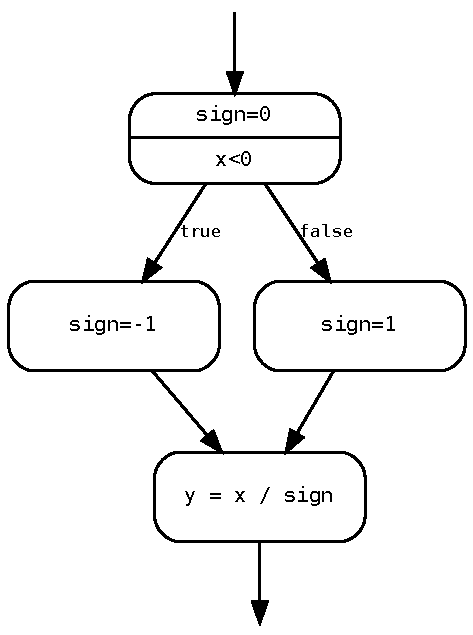
\includegraphics[height=0.8\textheight]{Graphs/Examples_ifExampleCFG.pdf}}}
			\only<2>{\put(170, -10.0){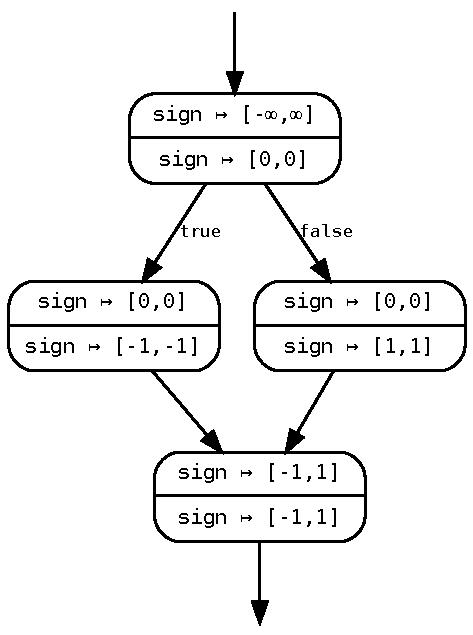
\includegraphics[height=0.8\textheight]{Graphs/Examples_ifExampleSign.pdf}}}
		\end{picture}
	\end{frame}

	% Semantics

	\begin{frame}[t]{Trace Partitioning Review}
		\begin{block}{Partitioned Semantics}
			Instead of classical implicit abstraction of trace semantics \concrete{P} to reachable states at position $l \in L$ with memory state $m \in M$ and further abstraction to abstract domain $D$,
			\begin{align}
				\concrete{P} \galois{\alpha_C}{\gamma_C} & (L \to M)\\
				& (L \to M) \galois{\alpha_D}{\gamma_D}  D 
			\end{align}
			extend first abstraction with \emph{covering} $\delta$ for arbitrary token set $T$
			\begin{align}
				\concrete{P} \galois{\alpha_\delta}{\gamma_\delta} & ((L \times T) \to M)\\
				& ((L \times T) \to M) \galois{\alpha_D}{\gamma_D}  D.
			\end{align}
		\end{block}
	\end{frame}

	% Partitioned States

	\begin{frame}[t]{Trace Partitioning Review}
		\begin{block}{Partitioned States}
			Rewrite partitioned reachable states as (curryfication):
			\begin{align}
				L \to (\underbrace{T \to M}_{\text{Partitioned State}})
			\end{align}
			Static analysis remains the same, considering now partitioned state instead of just memory state.
		\end{block}

		\begin{block}{Example State}
			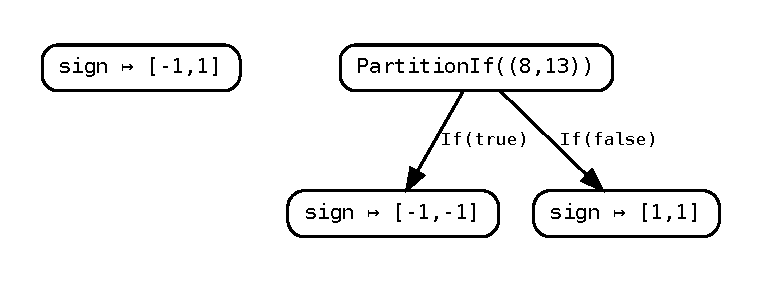
\includegraphics[width=\textwidth]{Graphs/PartitionedState.pdf}
		\end{block}
	\end{frame}

	% Tokens & Directives

	\begin{frame}[t]{Trace Partitioning Review}
		\begin{block}{Tokens}
			Represent decision made during the analysis. A token is either
			\begin{itemize}
				\item the empty token $\epsilon$,
				\item or a combination $t::t'$ of two tokens representing decisions.
			\end{itemize}
		\end{block}

		\begin{block}{Directives}
			Mechanism that partitions the state by generating the tokens. Represent the partitioning function.
		\end{block}

		\begin{block}{Example Directive}
			\code{PartitionIf} directive generates two new tokens.
			\begin{align}
				t \mapsto 
				\begin{cases}
					t::\code{If(true)}\\
					t::\code{If(false)}
				\end{cases}
			\end{align}
		\end{block}
	\end{frame}

	% Generating Directives & Widening

	\begin{frame}[t]{Trace Partitioning Review}
		\begin{block}{Where Do Directives Come From?}
			Manually inserted in the analysis. Possible future sources are
			\begin{itemize}
				\item annotations in code or
				\item heuristics that dynamically insert directives during analysis.
			\end{itemize}
		\end{block}

		\begin{block}{Why Not Just Rewrite Code?}
			Partitioning happens dynamically during analysis. \emph{Widening} limits the size of the tokens.
		\end{block}
	\end{frame}

\end{section}

% IMPLEMENTATION REVIEW

\begin{section}{Implementation Review}

	% State

	\begin{frame}[t]{Implementation Review}
		\begin{block}{Analysis State in Sample}
			A \code{State[S<:State[S]]} in \sample is a very generic analysis state used in the fixed point iteration (i.e. between statements/blocks). Each \code{State} provides lattice operations
			\begin{itemize}
				\item \code{lub(l:S, r:S):S} computing the least upper bound,
				\item \code{top():S} returning the top element of the lattice,
				\item ...
			\end{itemize}
			as well as semantic operations
			\begin{itemize}
				\item \code{assignVariable(x:SAV[S], r:SAV[S]):S} 
				\item \code{createObject(t:Type, p:ProgramPoint):S} 
				\item ...\\
			\end{itemize}
		\end{block}
	\end{frame}

	% GenericAbstractState & PartitionedState

	\begin{frame}[t]{Implementation Review}
		\begin{block}{Generic Abstract State}
			The default implementation of the \code{State} trait provided by \sample. Combines a heap analysis with some other semantic analysis. 
		\end{block}

		\begin{block}{Partitioned State}
			Main contribution of this project. Provides an alternative implementation of \code{State} that
			\begin{itemize}
				\item manages a \emph{guest domain} (e.g. \texttt{GenericAbstractState}),
				\item keeps track of the \emph{partitioning} (the tree structure) and 
				\item provides an interface to apply directives.
			\end{itemize}
			The
			\begin{itemize}
				\item \emph{lattice operations} are applied to the partitioning and
				\item \emph{semantic operations} are redirected to the guest domain states.
			\end{itemize}
		\end{block}
	\end{frame}

	% Architecture Overview

	\begin{frame}[t]{Implementation Review}
		\begin{block}{Architecture Overview}
			\begin{picture}(0.0,0.0)
				\put(-25.0,-150.0){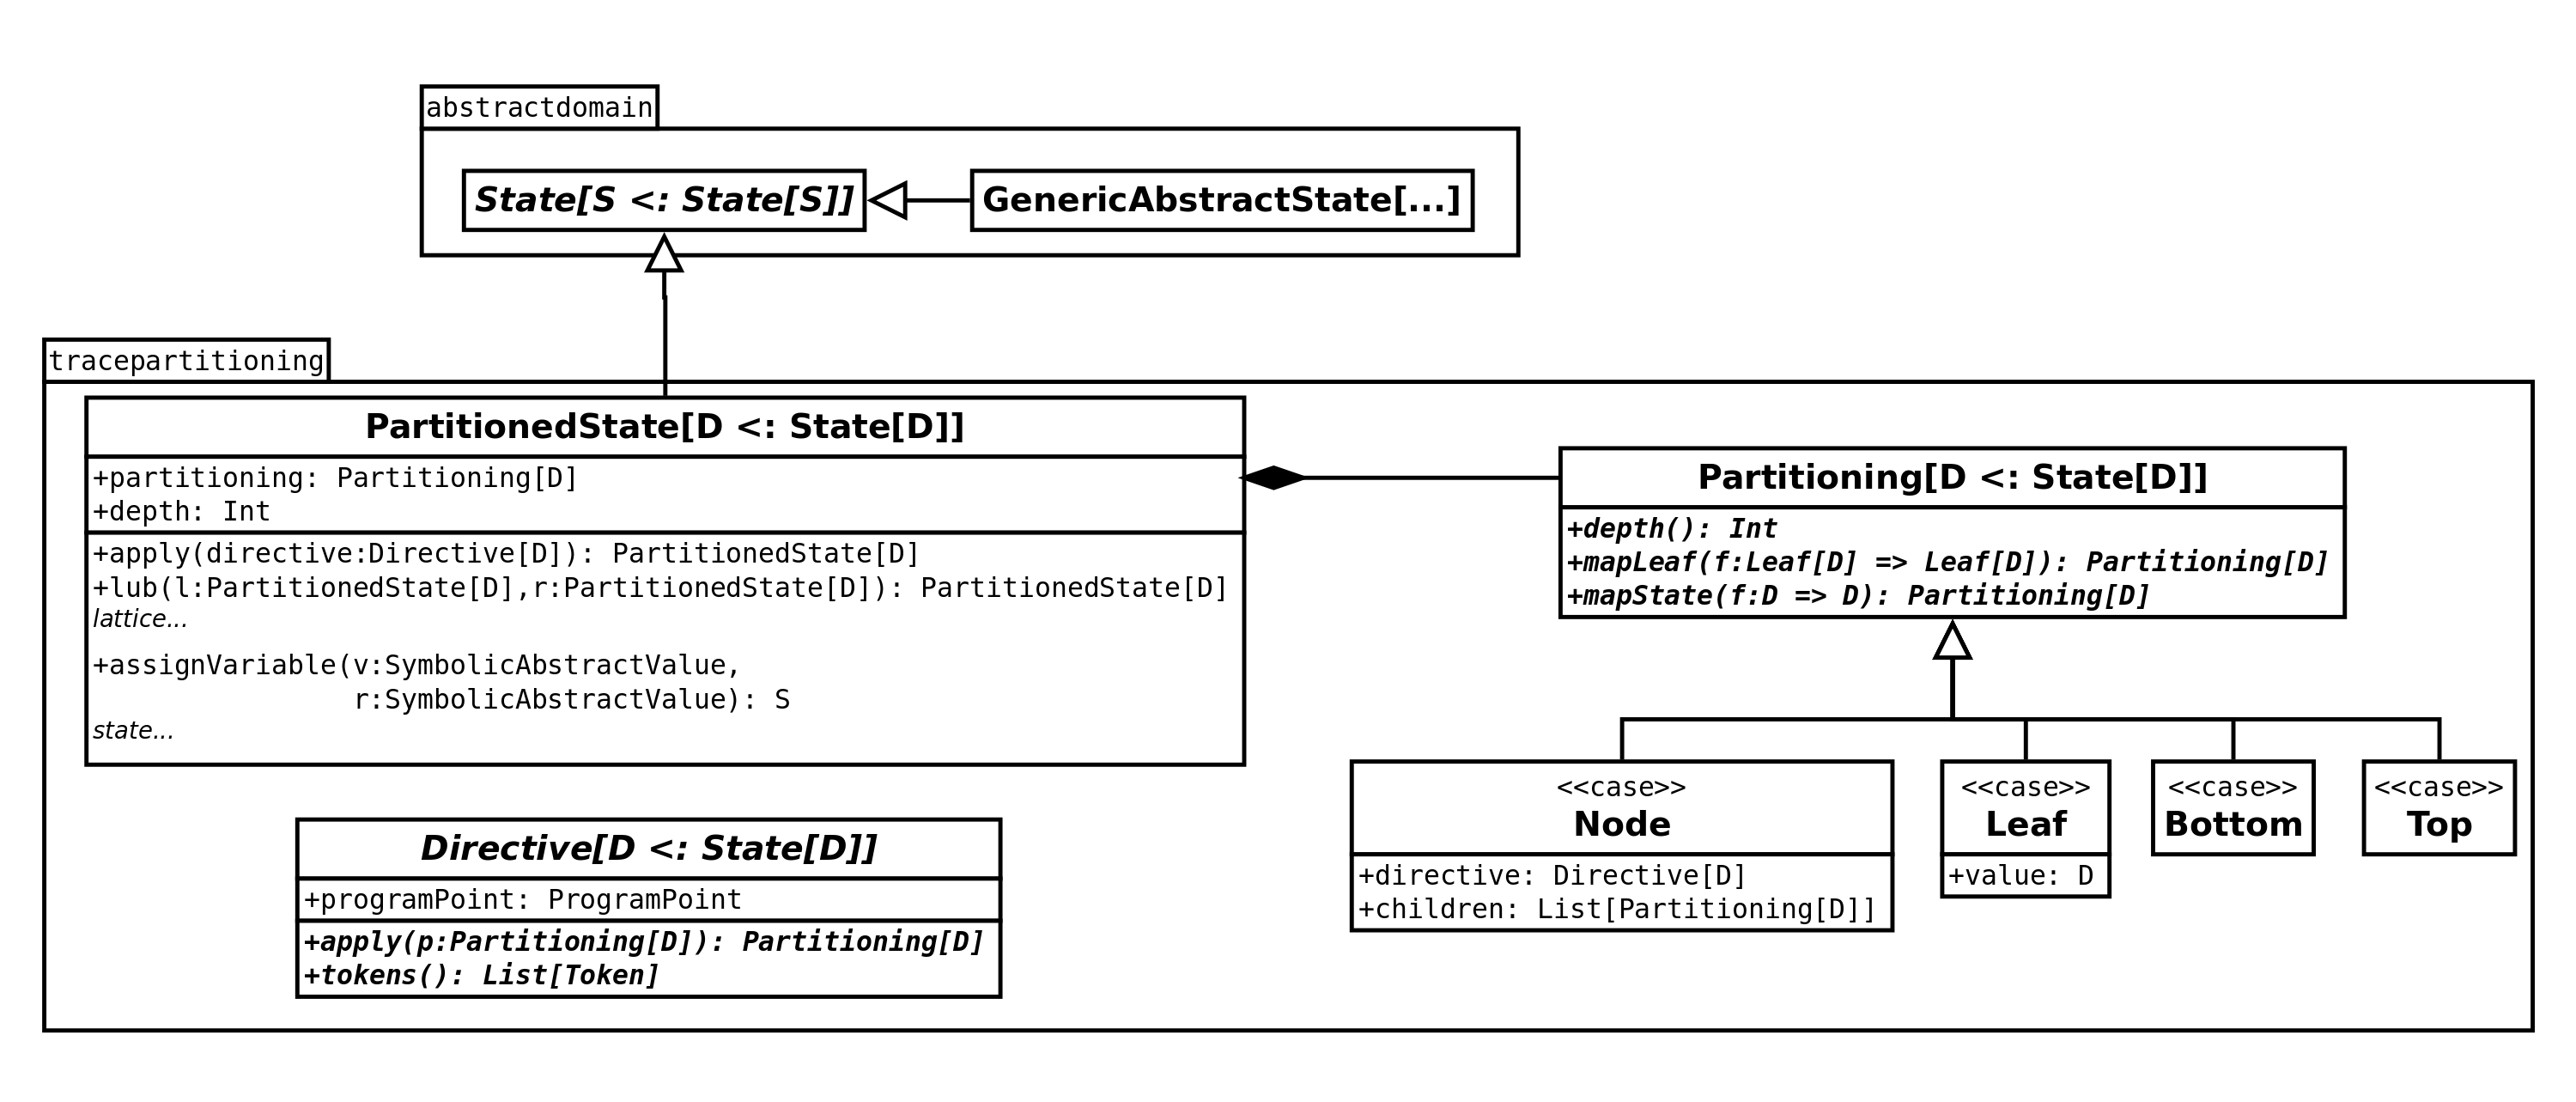
\includegraphics[width=12.5cm]{Diagrams/Architecture.png}}
			\end{picture}
		\end{block}
	\end{frame}

\end{section}

% DIRECTIVES

\begin{section}{Directives}

	% Overview

	\begin{frame}[t]{Directives}
		\begin{block}{Overview}
			The Directives implemented so far are:

			\begin{picture}(0.0,0.0)
				\put(-25.0,-150.0){\includegraphics[width=12.5cm]{Diagrams/Directive.png}}
			\end{picture}
		\end{block}
	\end{frame}

	% PartitionIf

	\begin{frame}[t]{Directives}
		\begin{block}{PartitionIf}
			Distinguishes traces based on whether or not they follow a conditional. \code{PartitionIf(pp)} generates the tokens \code{If(true)} and \code{If(false)}.

			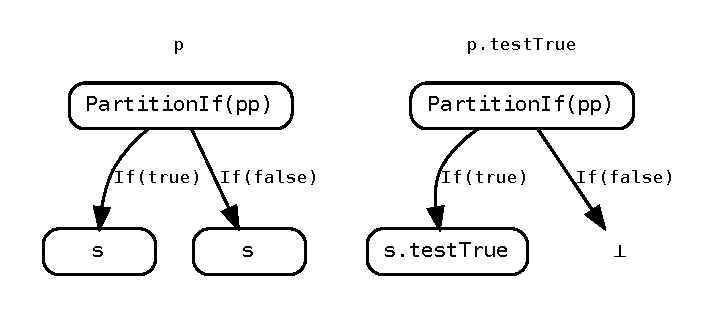
\includegraphics[width=\textwidth]{Graphs/PartitionIf.pdf}

			Assuming condition discards contradicted leaf.
		\end{block}
	\end{frame}

	% Merge

	\begin{frame}[t]{Directives}
		\begin{block}{Merge}
			Applies the inverse transformation of some other directive. \code{Merge(pp, source)} removes the generated tokens of the \code{source} directive and combines the leaves.

			\begin{center}
				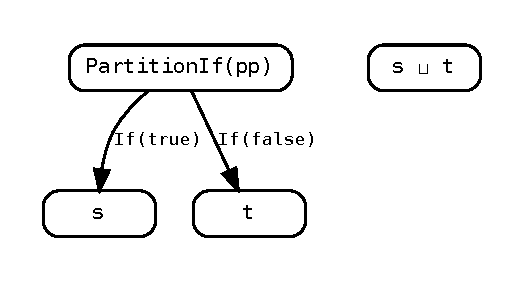
\includegraphics[scale=0.8]{Graphs/Merge.pdf}
			\end{center}

			Important to manage complexity of analysis.
		\end{block}
	\end{frame}

	% PartitionIf and Merge Example

	\begin{frame}[fragile, t]{Example}
		\begin{block}{Running Example}
			\lstinputlisting[]{Source/Examples_ifExample.scala}
		\end{block}

		\begin{block}{Property of Interest}
			Are all divisions safe?
		\end{block}
	\end{frame}

	% Non-Partitioned Analysis

	\begin{frame}[t]{Example}
		\begin{block}{Non-Partitioned Analysis}
			The conditional branch determining the value of \code{sign} generates states \code{p} and \code{q}.
			\begin{center}
				\includegraphics[scale=0.6]{Graphs/PartitionIfExample1.pdf}
			\end{center}
			Joining leads to the conclusion that \code{sign} could possibly be \code{0}.
		\end{block}
	\end{frame}

	% Partitioned Analysis

	\begin{frame}[t]{Example}
		\begin{block}{Partitioned Analysis}
			\only<1>{The conditional branch determining the value of \code{sign} generates states \code{p} and \code{q}.}
			\only<2>{Applying the \code{Merge} directive at the end of the method results a leaf state.}
			\begin{center}
				\only<1>{\includegraphics[width=\textwidth]{Graphs/PartitionIfExample2.pdf}}
				\only<2>{\includegraphics[scale=0.6]{Graphs/PartitionIfExample3.pdf}}
			\end{center}
			\only<1>{The upper bound is taken leaf-wise. The division will not generate a warning.}
		\end{block}
	\end{frame}

	% PartitionValue

	\begin{frame}[t]{Directives}
		\begin{block}{PartitionValue}
			Distinguishes between traces based on the value of some variable. \code{PartitionValue(pp, context)} generates tokens for conditions specified by helper object \code{context}.

			\begin{center}
				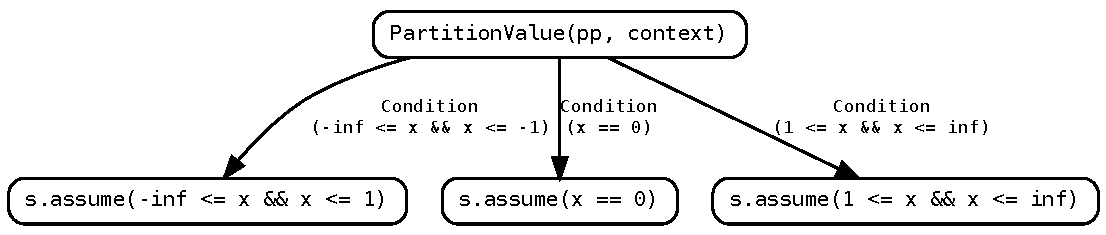
\includegraphics[width=\textwidth]{Graphs/PartitionValue.pdf}
			\end{center}
			
			Based on \code{PartitionCondition} which allows arbitrary conditions (as \code{Expression}) to be assumed.
		\end{block}
	\end{frame}

	% PartitionValue Example

	\begin{frame}[t]{Example}
		\begin{block}{Piecewise Linear Function}
			\begin{columns}
				\begin{column}{4cm}
					\begin{align*}
						y(x) =
							\begin{cases}
								-x - 1 & \text{if } x < -1\\
								x - 1 & \text{if } x > 1\\
								0 & \text{otherwise}
							\end{cases}
					\end{align*}
				\end{column}
				\begin{column}{5cm}
					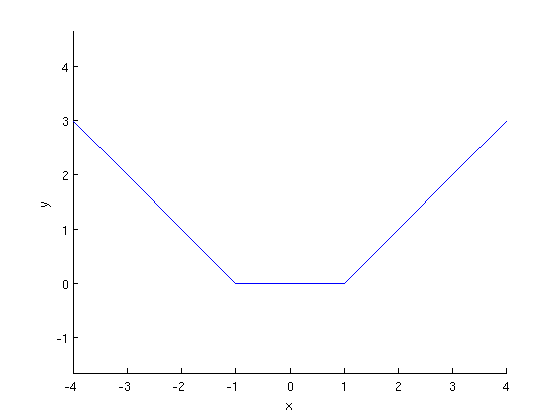
\includegraphics[scale=0.4]{Plots/valueExample.png}
				\end{column}
			\end{columns}
		\end{block}
		\begin{block}{Property of Interest}
			The analysis is interested in the range of the resulting \code{y}.
		\end{block}
	\end{frame}

	% Code

	\begin{frame}[t]{Example}
		\begin{block}{Evaluation}
			\lstinputlisting[]{Source/Examples_valueExample.scala}
			Analysis state after line \code{9} is crucial for the precision of the result.
		\end{block}
	\end{frame}

	% Non-partitioned Analysis

	\begin{frame}[t]{Example}
		\begin{block}{Non-Partitioned Analysis}
			The conditional branches determining the value of \code{i} generate states \code{p}, \code{q} and \code{r}.
			\begin{center}
				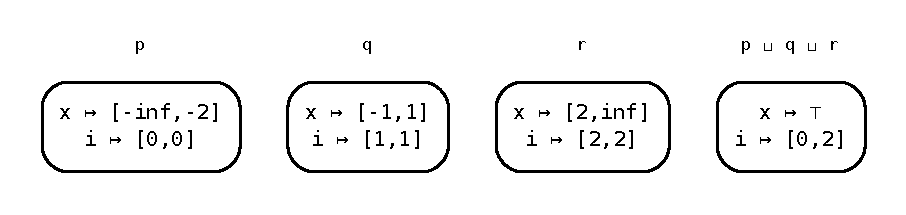
\includegraphics[scale=0.6]{Graphs/PartitionValueExample1.pdf}
			\end{center}
			Joining these states then leads to the conclusion that \code{y} must be in \code[-inf,inf].
		\end{block}
	\end{frame}

	% Partitioned Analysis

	\begin{frame}[t]{Example}
		\begin{block}{Partitioned Analysis}
			\only<1-3>{Using a \code{PartitionValue} directive, that partitions over values of \code{x} with intervals \code{[-inf,-2]}, \code{[-1,1]} and \code{[2,inf]} changes \code{p}, \code{q} and \code{r}.}
			\only<4>{The upper bound is taken leaf-wise.}
			\only<5>{Continuing the analysis ends with the state \code{s}.}
			\only<6>{Applying a \code{Merge} directive produces the desired result.}
			\begin{center}
				\only<1>{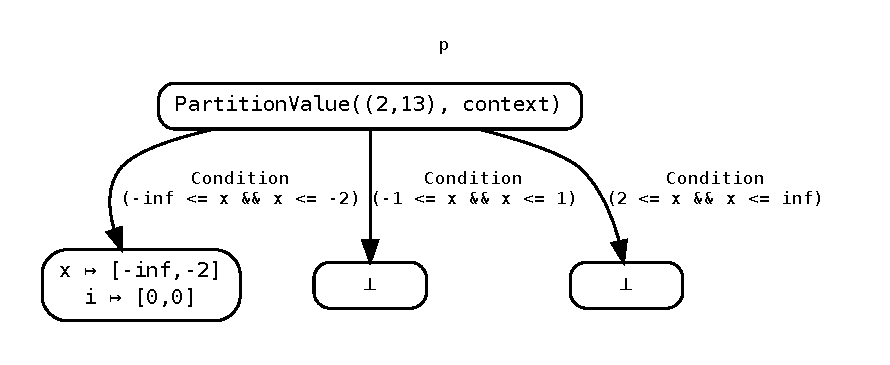
\includegraphics[scale=0.6]{Graphs/PartitionValueExample21.pdf}}
				\only<2>{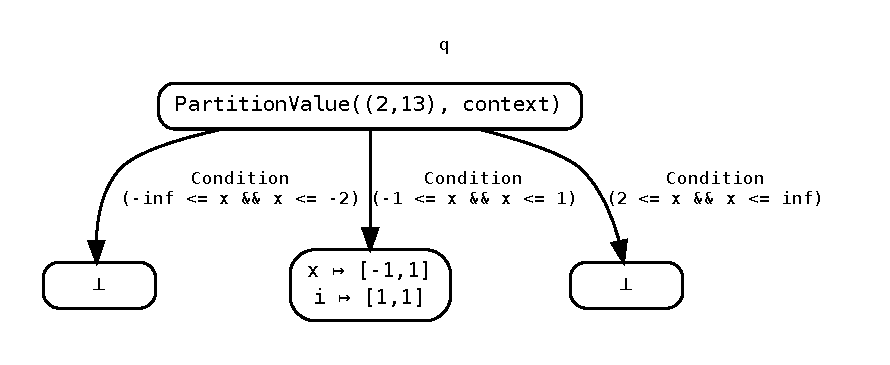
\includegraphics[scale=0.6]{Graphs/PartitionValueExample22.pdf}}
				\only<3>{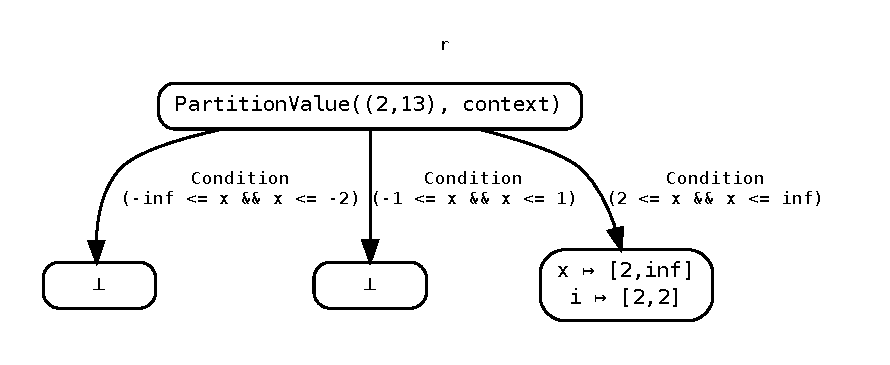
\includegraphics[scale=0.6]{Graphs/PartitionValueExample23.pdf}}
				\only<4>{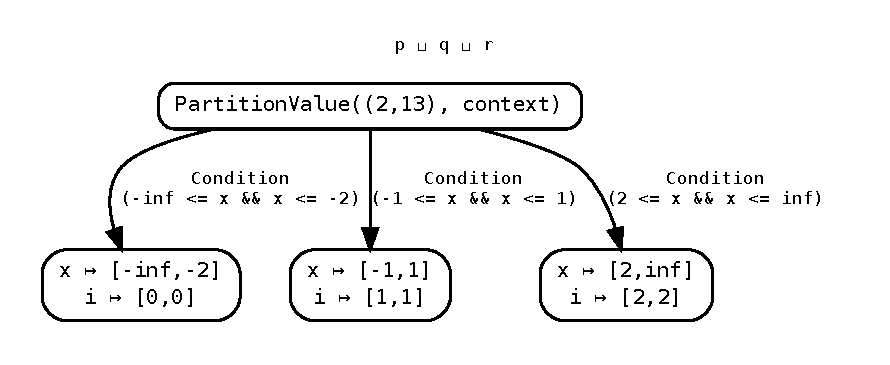
\includegraphics[scale=0.6]{Graphs/PartitionValueExample24.pdf}}
				\only<5>{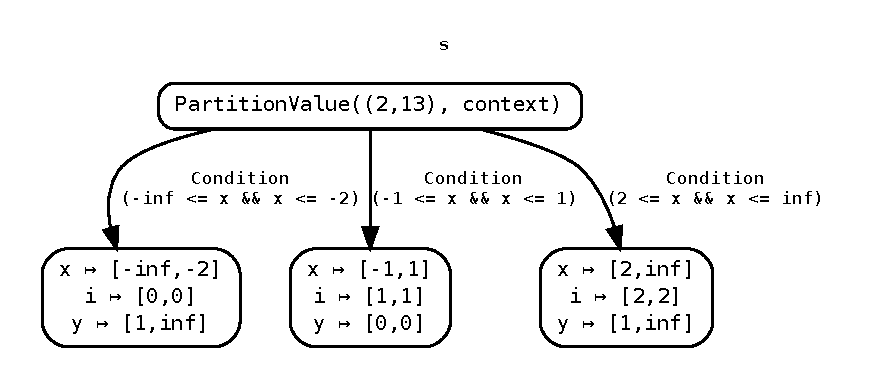
\includegraphics[scale=0.6]{Graphs/PartitionValueExample25.pdf}}
				\only<6>{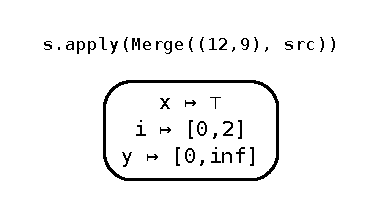
\includegraphics[scale=0.6]{Graphs/PartitionValueExample26.pdf}}
			\end{center}
		\end{block}
	\end{frame}

	% PartitionWhile

	\begin{frame}[t]{Directives}
		\begin{block}{PartitionWhile}
			Distinguishes traces based on how many times they traverse a loop. \code{PartitionWhile(pp, n)} generates for \code{i} from \code{0} to \code{n} tokens \code{While(i)} representing \code{i}, and \code{While(inf)} representing more than \code{n} traversals.

			\begin{center}
				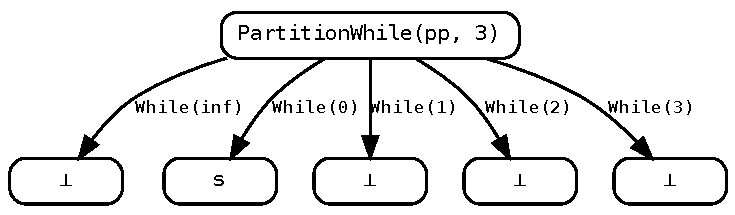
\includegraphics[width=\textwidth]{Graphs/PartitionWhile.pdf}
			\end{center}

			Tricky to implement.
		\end{block}
	\end{frame}

	\begin{frame}[t]{Example}
		\begin{block}{Iteration Index}
			\lstinputlisting[]{Source/Examples_whileExample.scala}
			Analysis with \code{PartitionWhile} directive generates the following result after line \code{5}.
			\begin{center}
				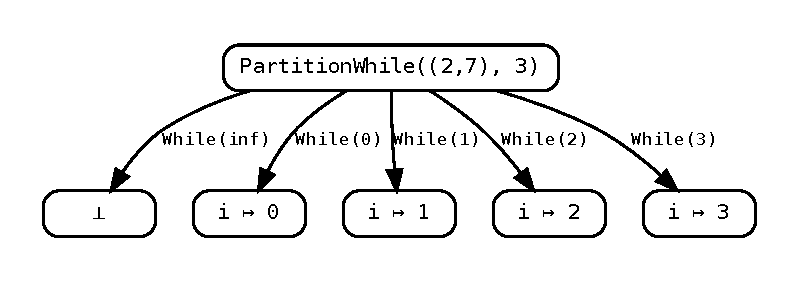
\includegraphics[width=\textwidth]{Graphs/PartitionWhileExample.pdf}
			\end{center}
		\end{block}
	\end{frame}

	% User Interface Demo

	\begin{frame}{Demo}
		\begin{center}
			\large{User Interface Demo}
		\end{center}
	\end{frame}

\end{section} 

% DISCUSSION

\begin{section}{Discussion}

	% Evaluation

	\begin{frame}[t]{Discussion}
		\begin{block}{Evaluation}
			Performance is difficult to assess. Highly dependent on choice of directives. Ignoring the widening, penalty for analysis can be
			\begin{itemize}
				\item \emph{constant}, e.g. with a \code{PartitionIf} in a cycle free context or
				\item \emph{exponential}, e.g. with a \code{PartitionIf} without merge inside a loop.
			\end{itemize}
			However, increased precision can also improve convergence of fixed point iteration.

			Both suggest doing analysis on a larger scale. Main obstacles for this currently are
			\begin{itemize}
				\item unavailable heuristics for directives and
				\item some features lacking in \sample (e.g. array access).
			\end{itemize}
		\end{block}
	\end{frame}

	% Open Questions & Possible Extensions

	\begin{frame}[t]{Discussion}
		\begin{block}{Open Questions}
			Main problem is, in my opinion, lack of heuristics to insert directives automatically. Coming up with heuristics ``obvious'' for simpler directives, for \code{PartitionValue} it is already quite tricky.
		\end{block}

		\begin{block}{Possible Extensions}
			Plenty of possibilities.
			\begin{itemize}
				\item Coming up with sensible heuristics. Implement heuristics mechanism.
				\item Implementing new directives, e.g. based on \code{PartitionCondition}.
				\item Domain specific directives, e.g. based on the heap domain (distinguish traces with/without aliasing). 
			\end{itemize}
		\end{block}
	\end{frame}

	% Conclusion

	\begin{frame}[t]{Discussion}
		\begin{block}{Conclusion}
			Generally happy with the outcome of a project that gave me the opportunity to 
			\begin{itemize}
				\item study a challenging and interesting subject,
				\item work on a bigger software project and
				\item at the same time learn a new language.
			\end{itemize}
			
			Contribution is arguably more groundwork than exploration. Nonetheless, I hope it will serve as basis for many future projects.
		\end{block}
	\end{frame}

	% Questions & Comments

	\begin{frame}{}
		\begin{center}
			\large{Questions? Comments!}
		\end{center}
	\end{frame}

\end{section}

\end{document}
